\documentclass{article}%
\usepackage[T1]{fontenc}%
\usepackage[utf8]{inputenc}%
\usepackage{lmodern}%
\usepackage{textcomp}%
\usepackage{lastpage}%
\usepackage[head=40pt,margin=0.5in,bottom=0.6in]{geometry}%
\usepackage{graphicx}%
%
\title{\textbf{Familiares de muertos en Torre Viasa llevarán caso a Fiscalía y Defensoría}}%
\author{SANDRA GUERRERO}%
\date{15/11/2018}%
%
\begin{document}%
\normalsize%
\maketitle%
\textbf{URL: }%
http://www.el{-}nacional.com/noticias/sucesos/familiares{-}muertos{-}torre{-}viasa{-}llevaran{-}caso{-}fiscalia{-}defensoria\_259783\newline%
%
\textbf{Periodico: }%
EN, %
ID: %
259783, %
Seccion: %
Sucesos\newline%
%
\textbf{Palabras Claves: }%
Sucesos\newline%
%
\textbf{Derecho: }%
1.1%
, Otros Derechos: %
1.10%
, Sub Derechos: %
1.1.1.9, 1.10.1.1%
\newline%
%
\textbf{EP: }%
NO\newline%
\newline%
%
\textbf{\textit{Los cadáveres no han sido entregados porque les harán reconocimiento post mórtem ante un juez y un fiscal}}%
\newline%
\newline%
%
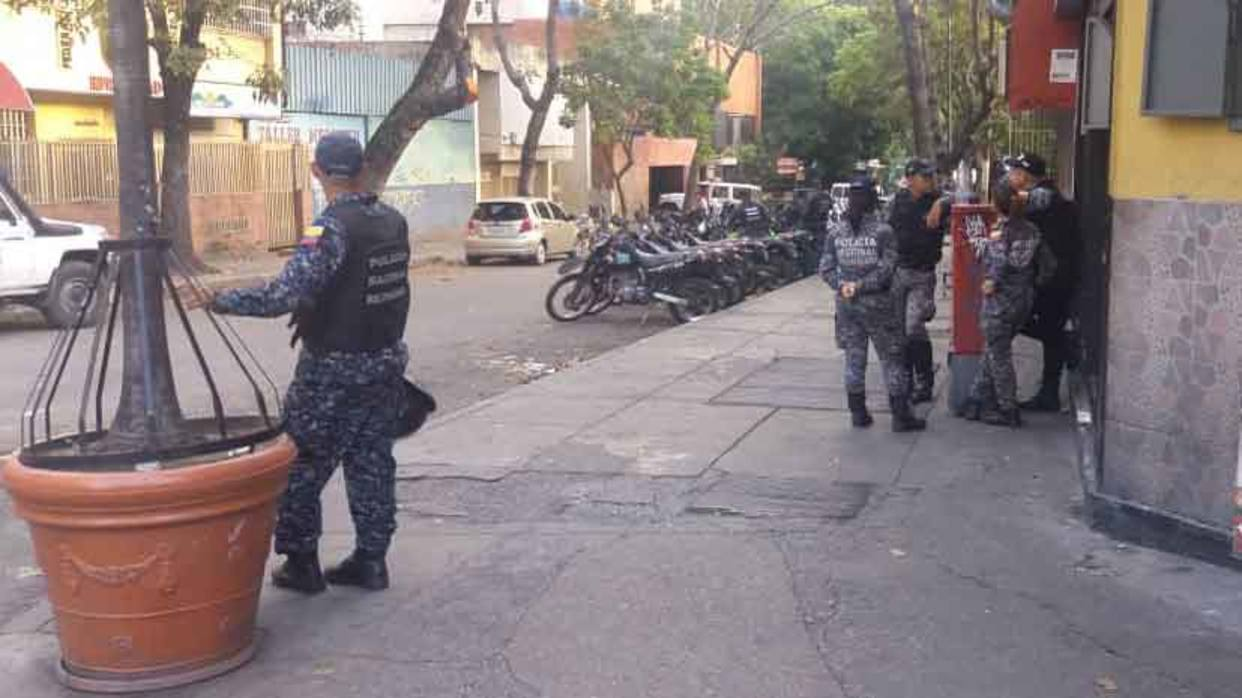
\includegraphics[width=300px]{204.jpg}%
\newline%
%
Los parientes de los siete fallecidos en la Torre Viasa, ultimados por una comisión de las FAES, denunciarán los hechos en la Fiscalía y Defensoría del Pueblo al considerar que ninguna de las víctimas se enfrentó, pues fueron escogidos por los policías en la planta baja y luego fueron llevados al piso 11 donde los mataron.%
\newline%
%
El operativo en la torre comenzó a las 12:30 de la tarde, media hora después de que se supo que el oficial agregado de PNB José Antonio Canales Alemán recibió un tiro en la cara para robarle la pistola, en la avenida Bolívar. Alguien dijo que los autores del hecho estaban en esa torre.%
\newline%
%
Familiares de los fallecidos denunciaron que están siendo amedrentados por la FAES y la PNB, que están dando vueltas en patrullas por el edificio.%
\newline%
%
A la única familia que ayer le habían entregado el acta de defunción fue a la de Asley Flores Rodríguez, de 41 años de edad, porque va a ser llevado a Cumaná, para sepultarlo. Murió a consecuencia de shock hipovolémico que le ocasionó hemorragia interna al recibir un tiro en el tórax.%
\newline%
%
Johan Alberto Mijares Izquiel, de 22 años de edad, llevaba 10 años viviendo en la torre desde que perdió su casa en el barrio Unión de Petare, a consecuencia de las lluvias. Era el noveno de 10 hermanos.%
\newline%
%
Ernesto Mijares, padre de Mijares Izquiel, dijo que había salido a hacer una compra y cuando regresó la torre estaba acordonada por los policías y no lo dejaron entrar. “El tiroteo comenzó a las 3:00 pm. Hicieron una masacre”, explicó.%
\newline%
%
Mijares Izquiel vendía tostones en Sabana Grande, era el noveno de 10 hermanos y padre de una niña. Le botaron sus documentos de identidad y el padre buscó una copia de la partida de nacimiento para reclamar el cadáver. Mijares dijo que su hijo estaba a presentación y tenía seis horas de trabajo comunitario.%
\newline%
%
Jhoani Roca Gil, técnico en teléfonos, evangélico, estaba en su casa cuidando a sus tres hijas. Era el mayor de tres hermanos.%
\newline%
%
Los cadáveres no habían sido entregados ayer a los parientes, porque van a ser sometidos a reconocimiento post mórtem, proceso que retardará la entrega de los cuerpos que entrarán en descomposición. En principio los familiares irán a la Fiscalía 125º en la que declararán en torno al caso.%
\newline%
%
\end{document}